\includepdf{CG.pdf}
\section*{Funciones radiales}
 \begin{align*}
R_{10}(r)&= \frac{2}{a_0^{\,3/2}}\,\exp\left(-\frac{r}{a_0}\right),\\[0.5ex]
R_{20}(r) &= \frac{2}{(2\,a_0)^{3/2}}\left(1-\frac{r}{2\,a_0}\right)
\exp\left(-\frac{r}{2\,a_0}\right),\\[0.5ex]
R_{21}(r)&= \frac{1}{\sqrt{3}\,(2\,a_0)^{3/2}}\,\frac{r}{a_0}\,
\exp\left(-\frac{r}{2\,a_0}\right),\\[0.5ex]
R_{30}(r)&= \frac{2}{(3\,a_0)^{3/2}}\left(1-
\frac{2\,r}{3\,a_0} + \frac{2\,r^2}{27\,a_0^{\,2}}\right)\exp\left(-\frac{r}{3\,a_0}\right),\\[0.5ex]
R_{31}(r) &= \frac{4\,\sqrt{2}}{9\,(3\,a_0)^{3/2}}\,\frac{r}{a_0}
\left(1-\frac{r}{6\,a_0}\right)\,\exp\left(-\frac{r}{3\,a_0}\right),\\[0.5ex]
R_{32}(r)&= \frac{2\,\sqrt{2}}{27\,\sqrt{5}\,(3\,a_0)^{3/2}}
\left(\frac{r}{a_0}\right)^2 \exp\left(-\frac{r}{3\,a_0}\right).
\end{align*}

\section*{Integrales triviales}
\begin{align*}
  \int_0^\infty x^n e^{-ax} \dd{x} &= \frac{n!}{a^{n+1}}
\end{align*}

\section*{Relaciones trigonométricas}
\begin{align*}
  \sin^2(x) &= \frac{ 1 - \cos(2x) }{2}  \\
  \sin(a)\sin(b) &= \frac{\cos(a-b)-\cos(a+b)}{2}
\end{align*}

\section*{Pozo cuadrado}
Siendo los límites $x\in(\frac{-a}{2},\frac{a}{2})$, obtenemos
\begin{align*}
\Psi_n &= \sqrt{\frac{2}{L}}\sin \left( \frac{n\pi(x+a/2)}{a} \right) \ \stackrel{x\in(0,a)}{\rightarrow} \ \sqrt{\frac{2}{L}}\sin \left( \frac{n\pi x}{a} \right) \\
  k_n &= \frac{n\pi}{a} \\
  E_n &= \frac{\hbar^2k^2}{2m} = \frac{n^2 \hbar^2\pi^2}{2ma^2}
\end{align*}

\section*{Oscilador armónico}
\begin{align*}
  \psi_n(x) &= \frac{1}{\sqrt{2^n n!}} \left( \frac{m\omega}{\pi \hbar}
  \right)^{1/4} e^{\frac{-m\omega x^2}{2 \hbar}} H_n \left( \sqrt{
      \frac{m\omega}{\hbar}} x \right), \ \ n = \mathbb{Z}^+ \\
  E_n &= \hbar\omega \left( n + \frac{1}{2} \right)
\end{align*}

\section*{Hidrógeno}
La diferencia de energías entre niveles es
\begin{equation*}
  \Delta E = \SI{13.6}{\eV} \left( \frac{1}{n_f^2} - \frac{1}{n_i^2} \right)
\end{equation*}

La longitud de onda entre dos niveles es
\begin{equation*}
  \frac{1}{\lambda_\text{vac}} = R_H \left( \frac{1}{n_f^2} - \frac{1}{n_i^2} \right)
\end{equation*}

donde $R_H \simeq \SI{1.097e7}{\per\metre}$

\section*{Teorema del virial}
\begin{center}
  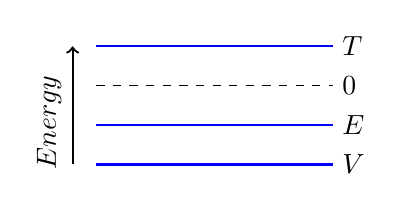
\begin{tikzpicture}[xscale=1.5,yscale=0.5]
    \draw [color=blue, thick] (0,1) -- (2,1); \draw node [right] at
    (2,1) {$T$};
    % 
    \draw [thin, dashed] (0,0) -- (2,0); \draw node [right] at (2,0)
    {$0$};
    % 
    \draw [color=blue, thick] (0,-1) -- (2,-1); \draw node [right] at
    (2,-1) {$E$};
    % 
    \draw [color=blue, thick] (0,-2) -- (2,-2); \draw node [right] at
    (2,-2) {$V$};
    % 
    \draw [thick,->] (-0.2,-2) -- (-0.2,1); \draw node [left,
    rotate=90] at (-0.4,0.5) {$\text{Energy}$};
  \end{tikzpicture}
\end{center}




%%% Local Variables:
%%% mode: latex
%%% TeX-master: "../resumen"
%%% End:
